\documentclass{article}
\usepackage{tikz}
\usetikzlibrary{positioning}

\begin{document}

\begin{figure}[h]
    \centering
    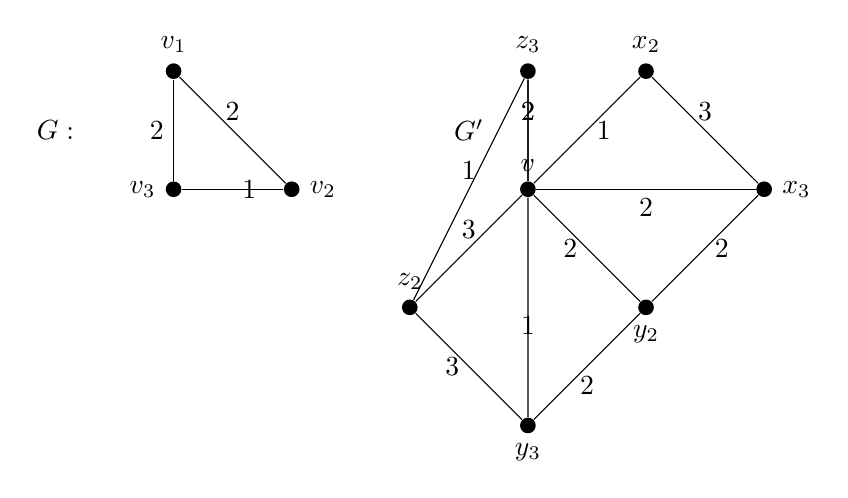
\begin{tikzpicture}[scale=1.5]
        % Define nodes for G
        \node[circle,fill,inner sep=2pt,label=above:$v_1$] (v1) at (0,1) {};
        \node[circle,fill,inner sep=2pt,label=right:$v_2$] (v2) at (1,0) {};
        \node[circle,fill,inner sep=2pt,label=left:$v_3$] (v3) at (0,0) {};
        
        % Draw edges with labels for G
        \draw (v1) -- node[above] {2} (v2);
        \draw (v2) -- node[right] {1} (v3);
        \draw (v3) -- node[left] {2} (v1);
        
        % Label G
        \node at (-1,0.5) {$G:$};
        
        % Define nodes for G'
        \node[circle,fill,inner sep=2pt,label=above:$x_2$] (x2) at (4,1) {};
        \node[circle,fill,inner sep=2pt,label=right:$x_3$] (x3) at (5,0) {};
        \node[circle,fill,inner sep=2pt,label=below:$y_2$] (y2) at (4,-1) {};
        \node[circle,fill,inner sep=2pt,label=below:$y_3$] (y3) at (3,-2) {};
        \node[circle,fill,inner sep=2pt,label=above:$z_2$] (z2) at (2,-1) {};
        \node[circle,fill,inner sep=2pt,label=above:$z_3$] (z3) at (3,1) {};
        \node[circle,fill,inner sep=2pt,label=above:$v$] (v) at (3,0) {};
        
        % Draw edges with labels for G'
        \draw (x2) -- node[above] {3} (x3);
        \draw (x3) -- node[right] {2} (y2);
        \draw (y2) -- node[below] {2} (y3);
        \draw (y3) -- node[left] {3} (z2);
        \draw (z2) -- node[above] {1} (z3);
        \draw (z3) -- node[above] {2} (v);
        \draw (v) -- node[right] {1} (x2);
        \draw (v) -- node[below] {2} (x3);
        \draw (v) -- node[left] {2} (y2);
        \draw (v) -- node[below] {1} (y3);
        \draw (v) -- node[above] {3} (z2);
        \draw (v) -- node[above] {2} (z3);
        
        % Label G'
        \node at (2.5,0.5) {$G'$};
    \end{tikzpicture}
\end{figure}

\end{document}